% !TEX root = manuscript.tex

\chapter*{Annexes}

\section*{Annexe 1: Détails techniques complémentaires}

\begin{itemize}
\item Langage de programmation : Python 3.9
\item IDE utilisé : Jupyter Notebook
\item Bibliothèques principales :
\begin{itemize}
\item TensorFlow 2.8.0
\item Keras 2.8.0
\item NumPy 1.22.3
\item Pandas 1.4.2
\item Scikit-learn 1.0.2
\item Matplotlib 3.5.1
\item Seaborn 0.11.2
\end{itemize}
\item Temps d'exécution détaillés
\begin{itemize}
\item Prétraitement des données : 2 minutes
\item Entraînement du MLP : 4 minutes (16 époques)
\item Entraînement du CNN simple : 6 minutes (11 époques)
\item Entraînement du CNN profond : 15 minutes (30 époques)
\item Génération des prédictions sur l'ensemble de test : 10 secondes
\end{itemize}
\end{itemize}


\section*{Annexe 2: Architecture du Perceptron}
\label{sec:annexe2}
\begin{figure}[H]
\centering
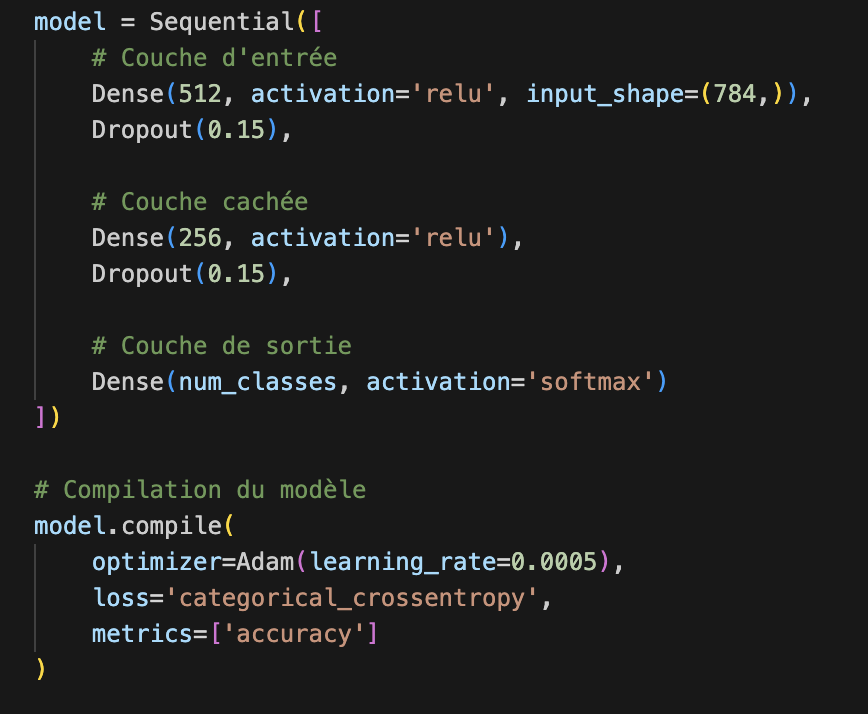
\includegraphics[width=0.5\textwidth]{figures/ArchiMLP.png}
\caption{Architecture du Perceptron.}
\label{fig:Architecture CNN Simple}
\end{figure}



\section*{Annexe 3: Architecture CNN Simple}
\label{sec:annexe3}
\begin{figure}[H]
\centering
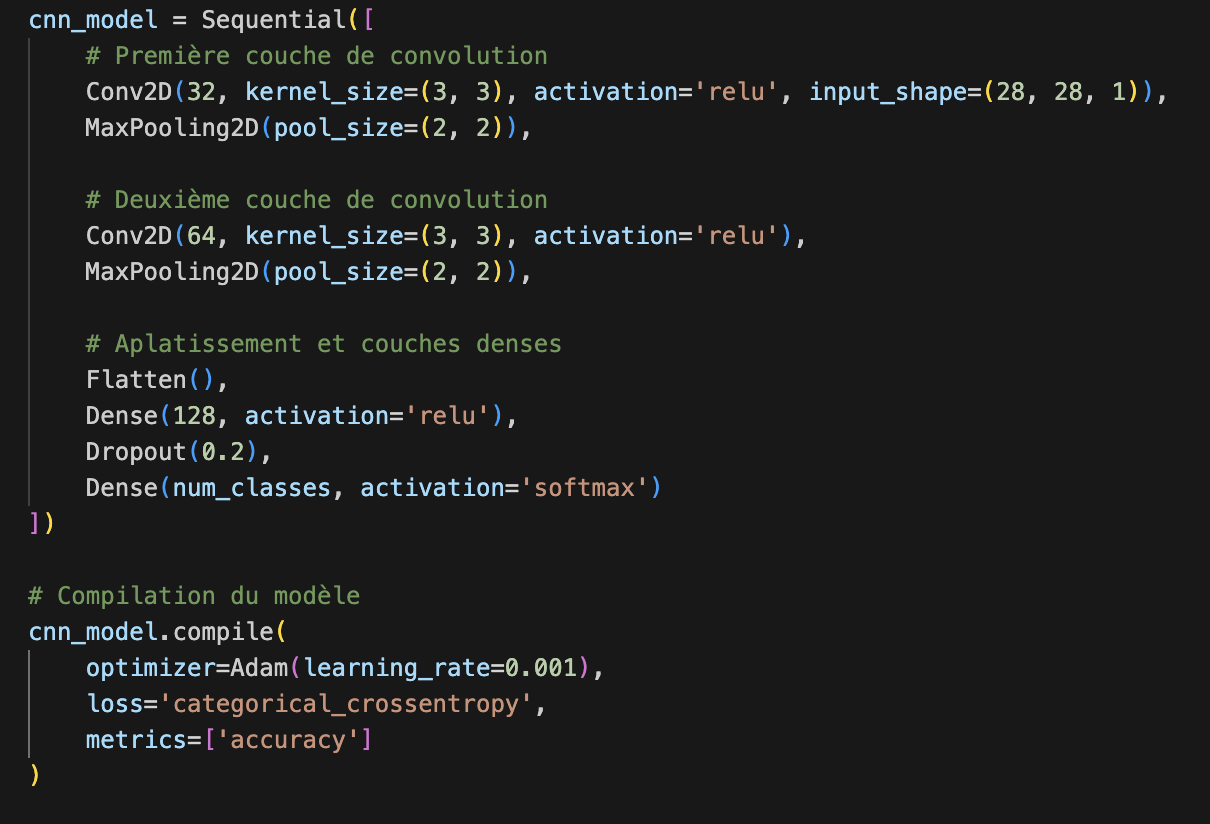
\includegraphics[width=0.5\textwidth]{figures/ArchiCNNSIMPL.png}
\caption{Architecture CNN Simple.}
\label{fig:Architecture CNN Simple}
\end{figure}




\section*{Annexe 4: Code source des principales fonctions}
\label{sec:annexe2}
\begin{itemize}
\item Prétraitement des données
\begin{figure}[H]
\centering
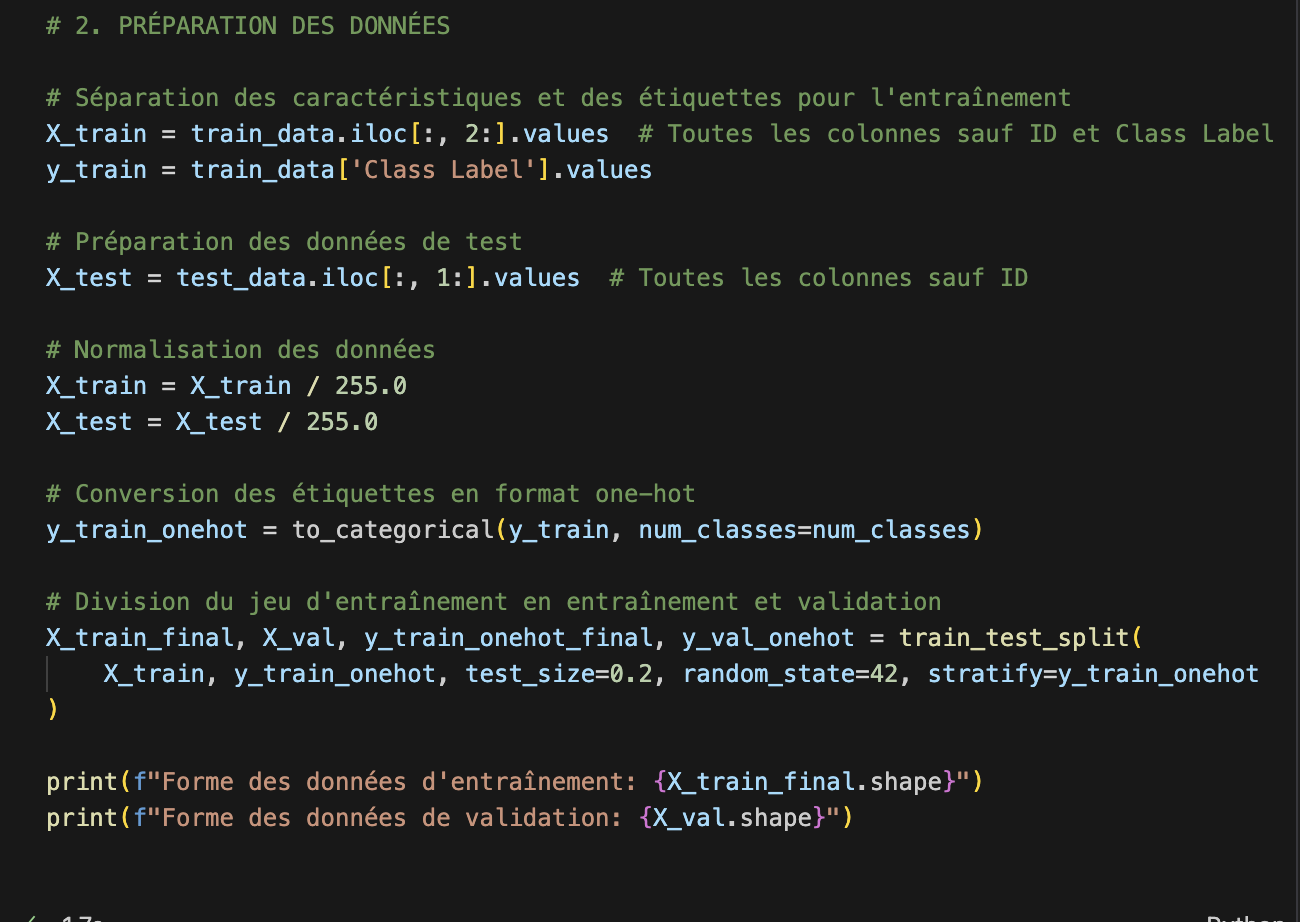
\includegraphics[width=0.5\textwidth]{figures/annexePre.png}
\caption{Code Pré traitement des données.}
\label{fig:Prétraitement des données}
\end{figure}
\item Visualisation des résultats
\begin{figure}[H]
\centering
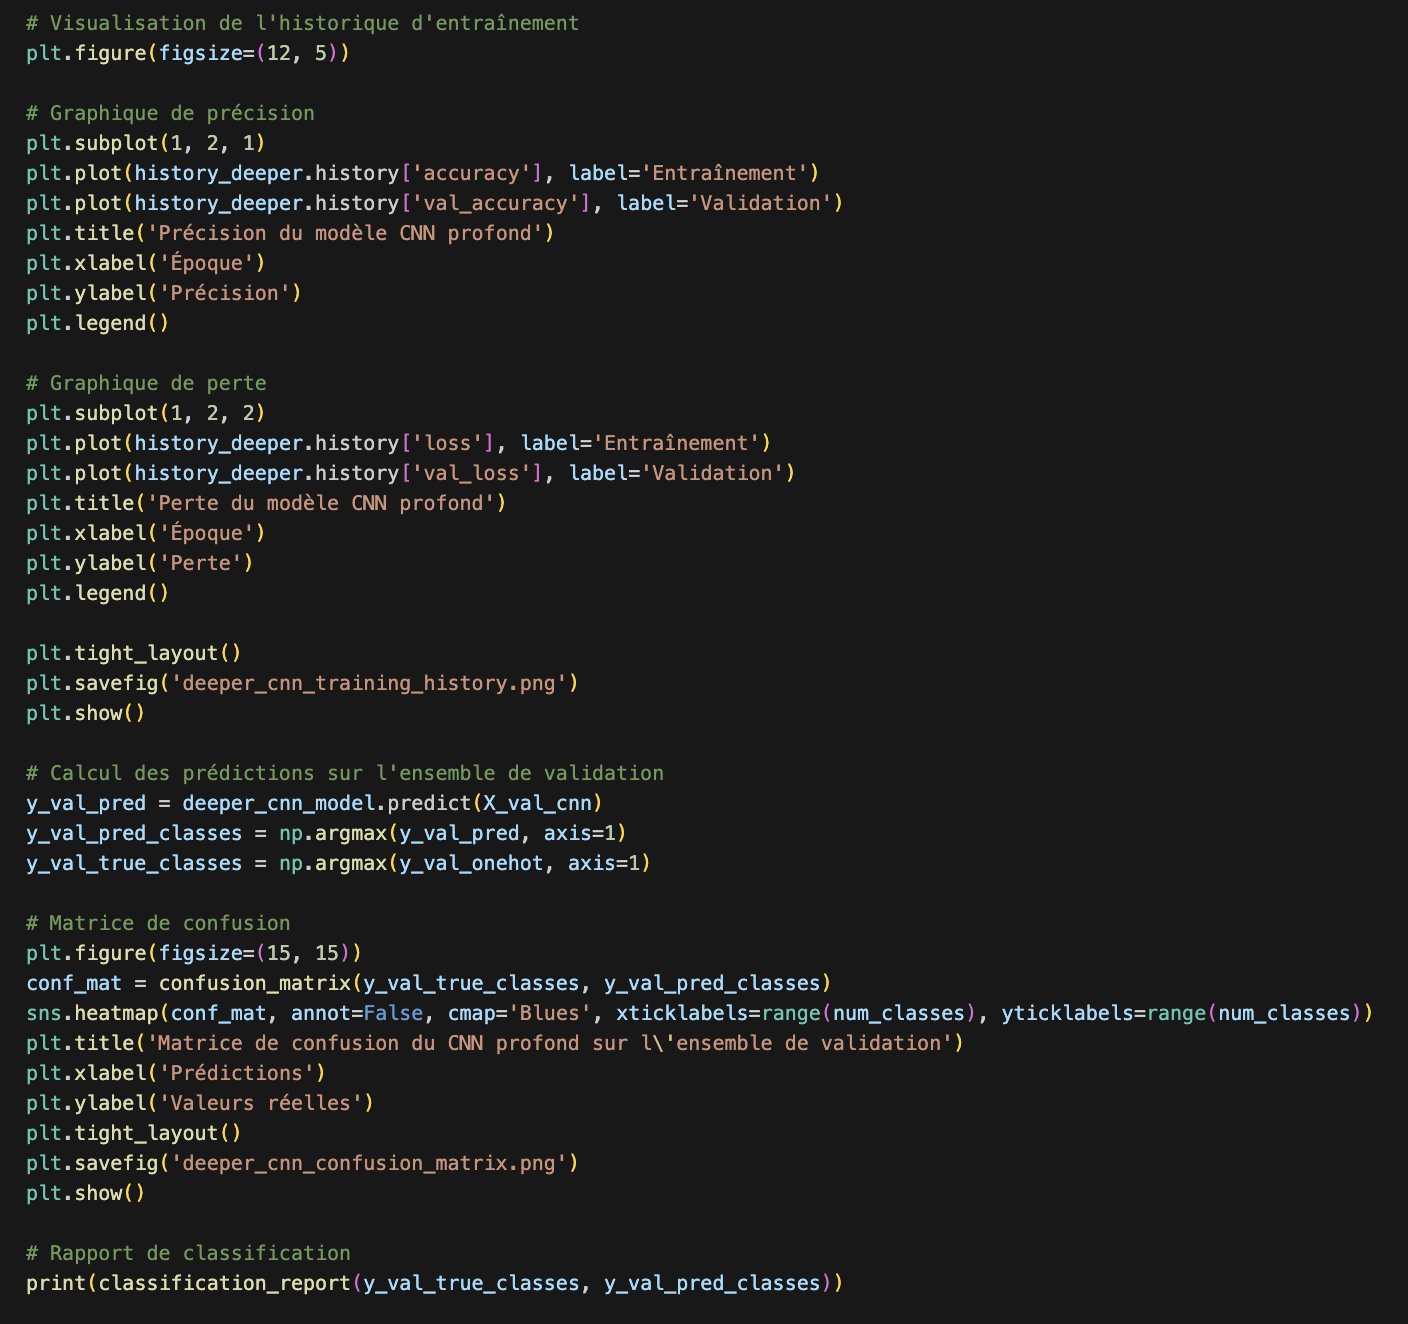
\includegraphics[width=0.5\textwidth]{figures/annexeVisua.png}
\caption{Code de visualisation des résultats.}
\label{fig:annexeVisua}
\end{figure}
\end{itemize}


\section*{Annexe 5: Annexe MLP}
\label{sec:annexe5}
\begin{itemize}
\item Précision et Perte du modèle
\begin{figure}[H]
\centering
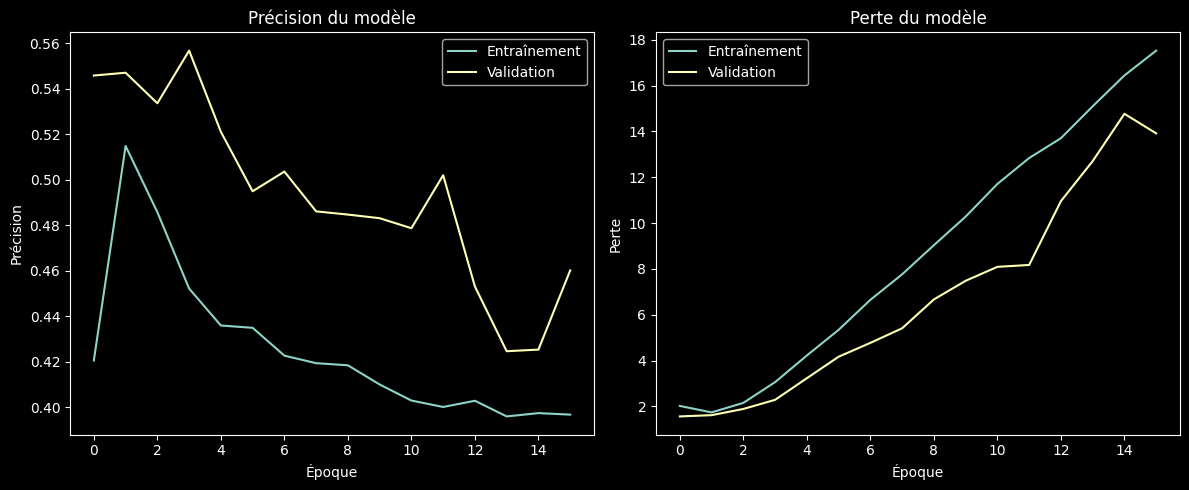
\includegraphics[width=0.5\textwidth]{figures/MLP1.png}
\caption{Courbe de précision et de perte.}
\label{fig:annexe5.1}
\end{figure}
\item Matrice de confusion
\begin{figure}[H]
\centering
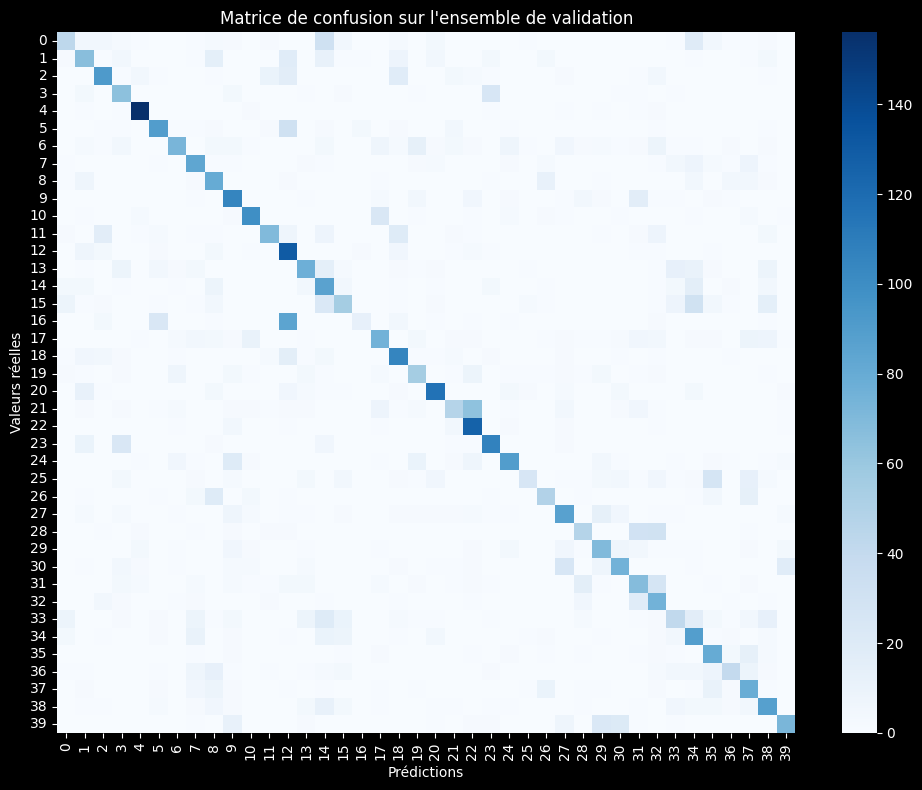
\includegraphics[width=0.5\textwidth]{figures/MLP2.png}
\caption{Matrice de confusion.}
\label{fig:annexe5.2}
\end{figure}
\item Résumé statistique du modèle
\begin{figure}[H]
\centering
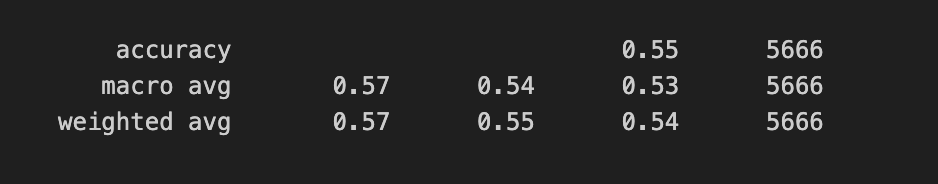
\includegraphics[width=0.5\textwidth]{figures/MLP3.png}
\caption{Résumé Statistique du modèle MLP.}
\label{fig:annexe5.3}
\end{figure}
\end{itemize}


\section*{Annexe 6: Modèle CNN Simple}
\label{sec:annexe6}
\begin{itemize}
\item Précision et Perte du modèle
\begin{figure}[H]
\centering
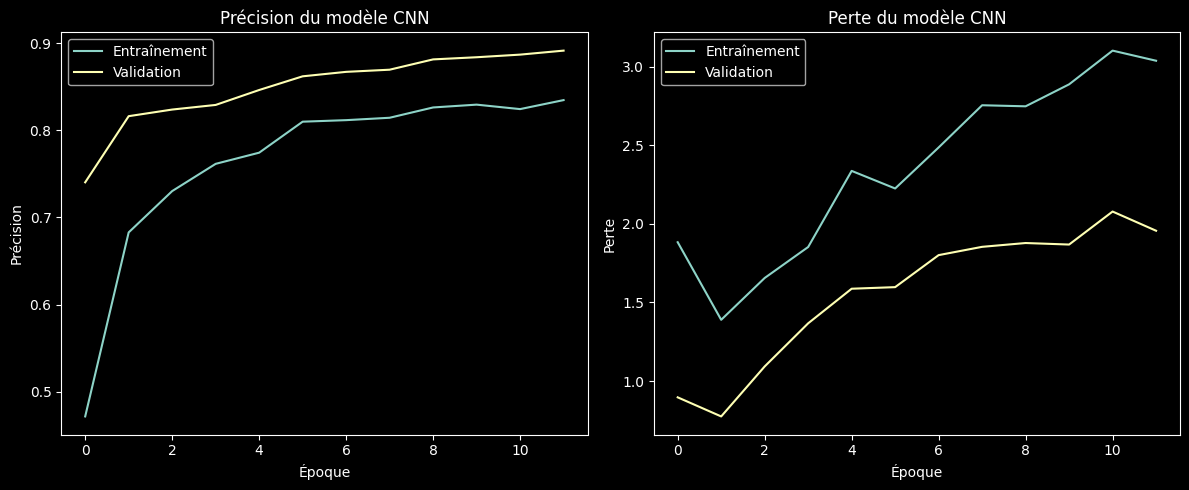
\includegraphics[width=1\textwidth]{figures/CNNSIMPLE1.png}
\caption{Courbe de précision et de perte.}
\label{fig:annexe6.1}
\end{figure}
\item Matrice de confusion
\begin{figure}[H]
\centering
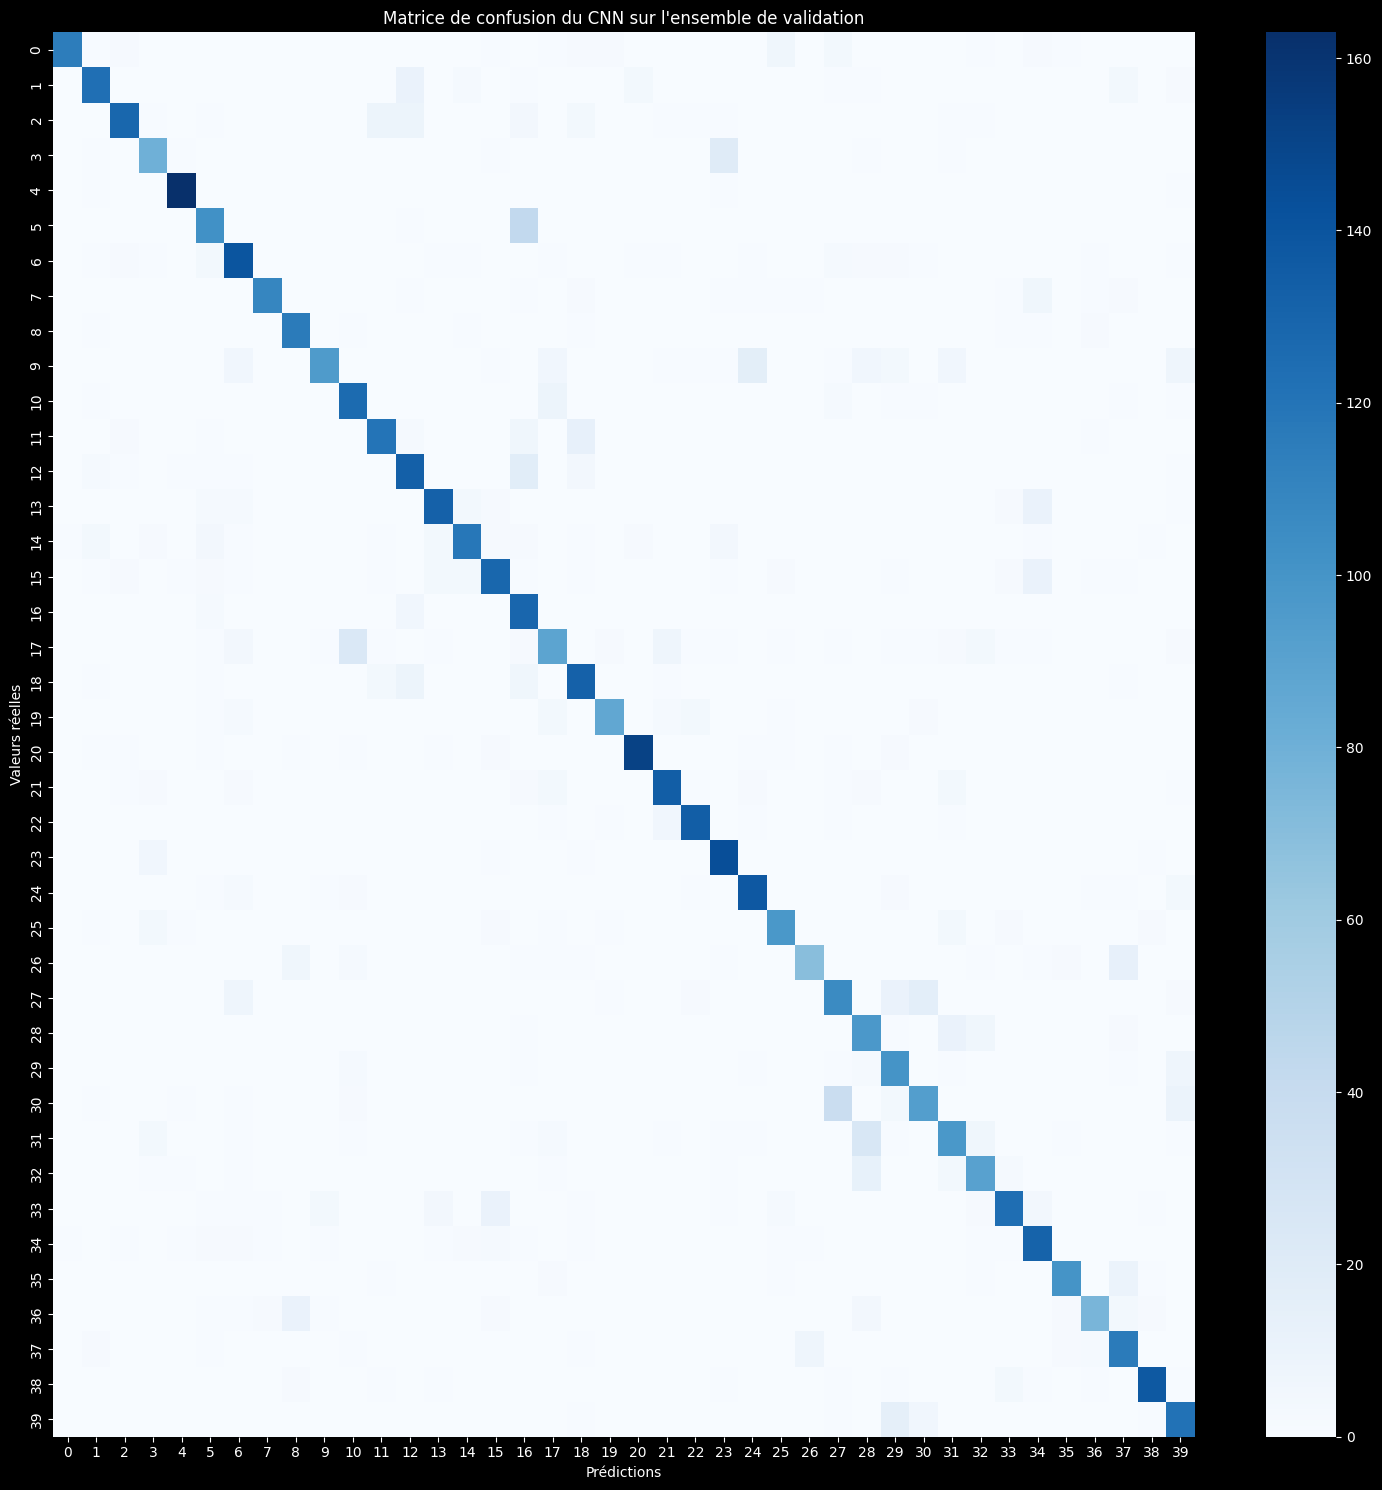
\includegraphics[width=0.5\textwidth]{figures/CNNSIMPLE2.png}
\caption{Matrice de confusion.}
\label{fig:annexe6.2}
\end{figure}
\item Résumé statistique du modèle
\begin{figure}[H]
\centering
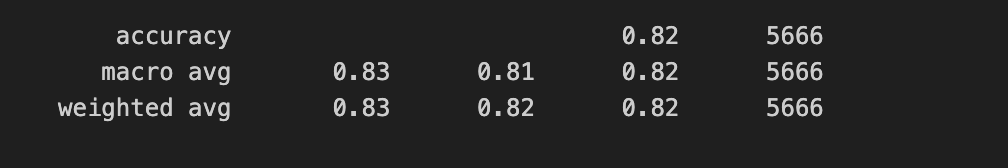
\includegraphics[width=0.5\textwidth]{figures/CNNSIMPLE3.png}
\caption{Résumé Statistique du modèle CNN Simple.}
\label{fig:annexe6.3}
\end{figure}
\end{itemize}



\section*{Annexe 7: Modèle CNN Profonde}
\label{sec:annexe7}
\begin{itemize}
\item Précision et Perte du modèle
\begin{figure}[H]
\centering
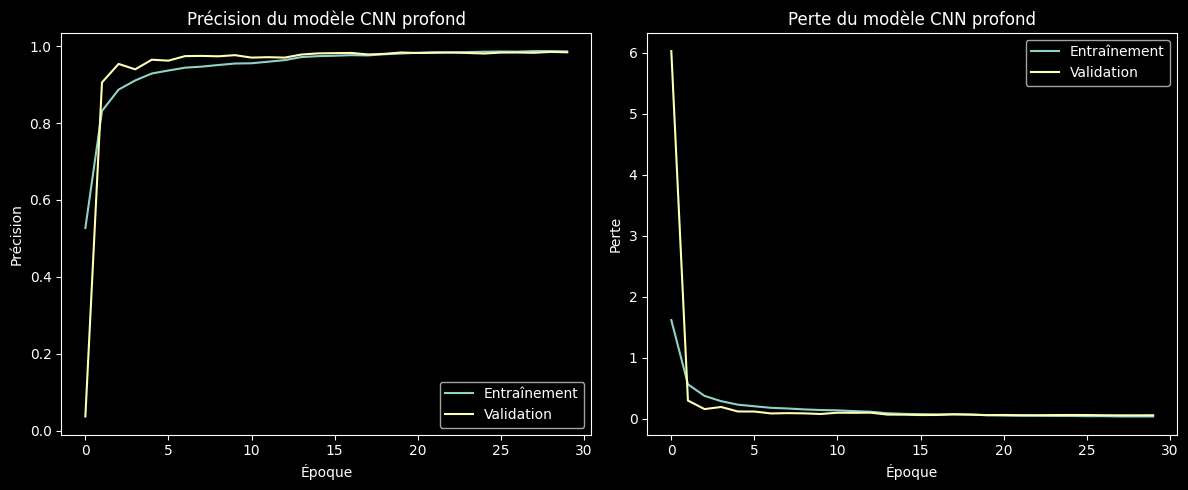
\includegraphics[width=1\textwidth]{figures/CNNPRO1.png}
\caption{Courbe de précision et de perte.}
\label{fig:annexe7.1}
\end{figure}
\item Matrice de confusion
\begin{figure}[H]
\centering
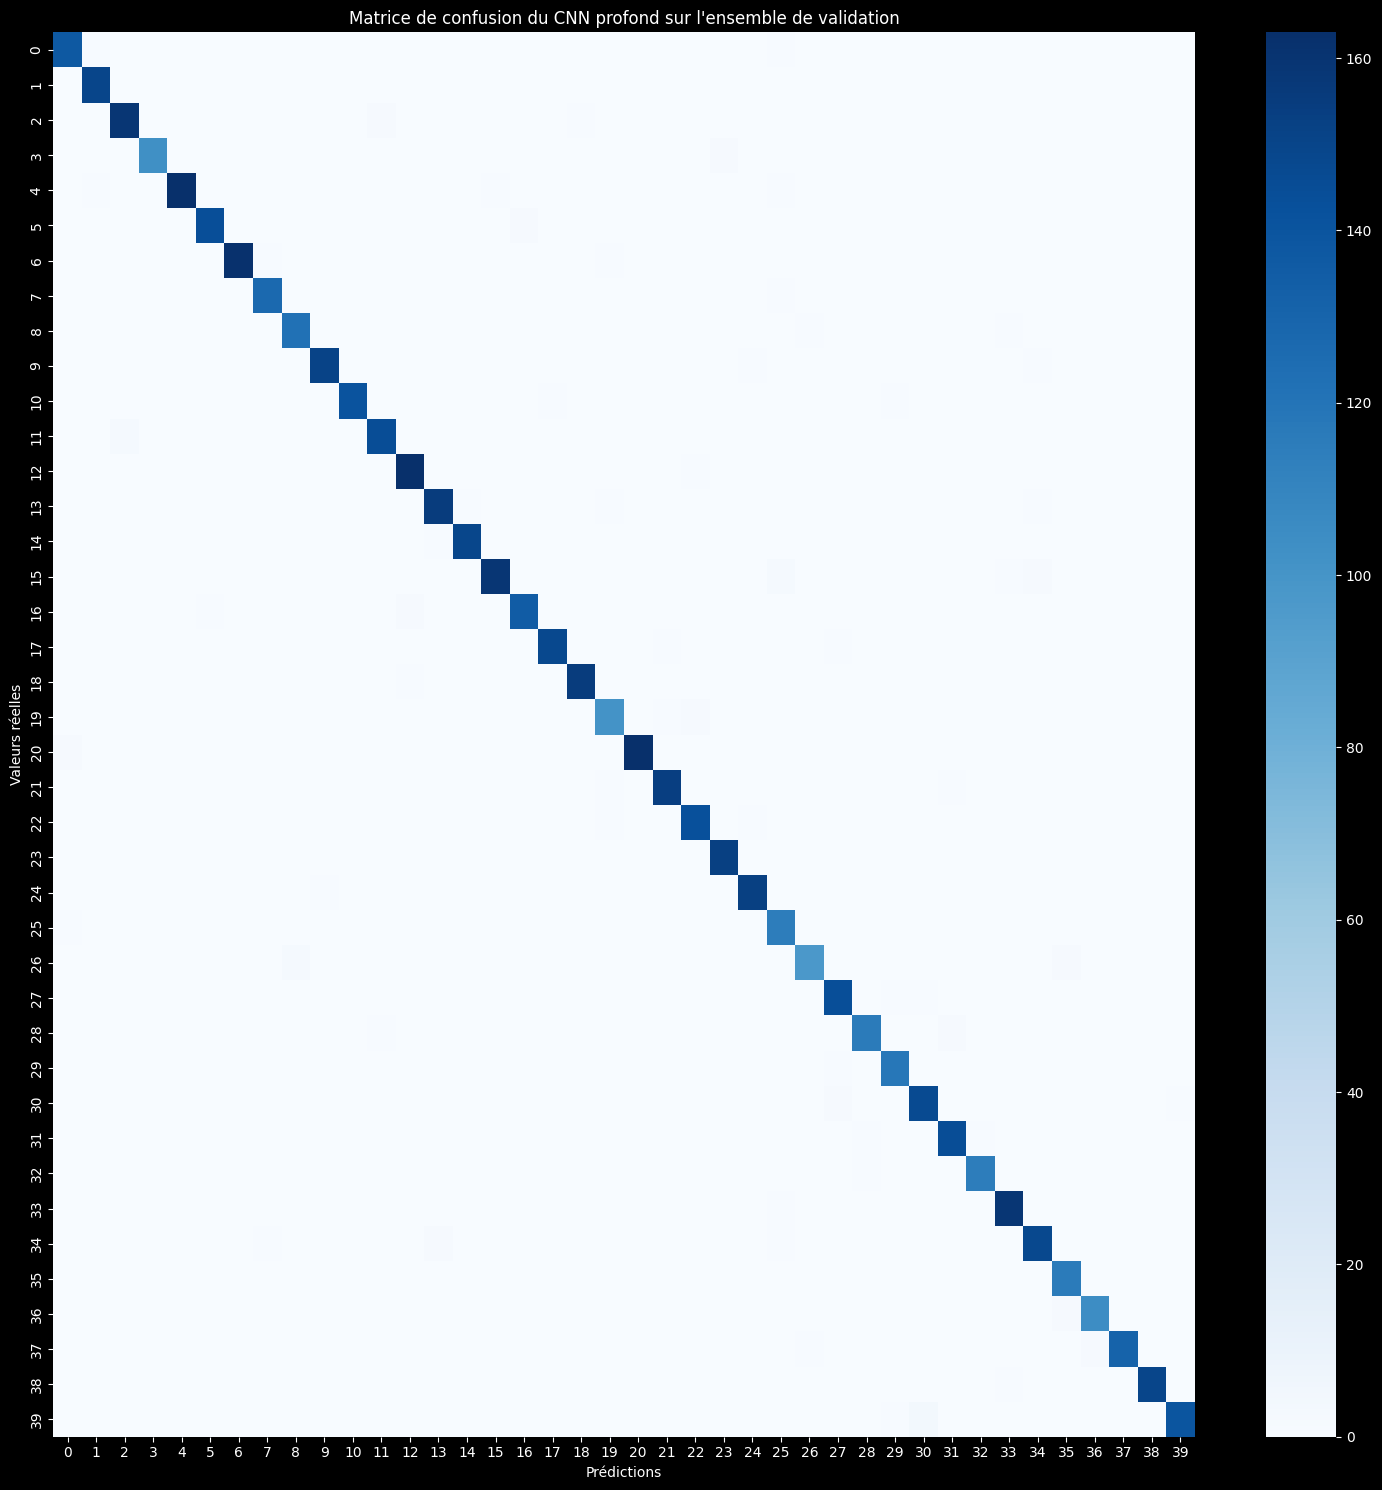
\includegraphics[width=0.5\textwidth]{figures/CNNPRO2.png}
\caption{Matrice de confusion.}
\label{fig:annexe7.2}
\end{figure}
\item Résumé statistique du modèle
\begin{figure}[H]
\centering
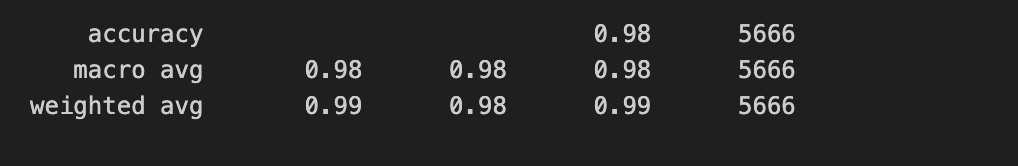
\includegraphics[width=0.5\textwidth]{figures/CNNPRO3.png}
\caption{Résumé Statistique du modèle CNN Profonde.}
\label{fig:annexe7.3}
\end{figure}
\end{itemize}


